\documentclass[aspectratio=169]{beamer}

	\usepackage{standalone}
	\usepackage{tikz}
	\usepackage{pgfplots}

	\usepackage{tabularray} % Typeset tabulars and arrays (contains equivalent of longtable, booktabs and dcolumn at least) 
		\UseTblrLibrary{booktabs} % to load extra commands from booktabs

	\usepackage{natbib}
\begin{filecontents*}[overwrite]{pres.bib}
@article{Knuth92,
	author = "D.E. Knuth",
	title = "Two notes on notation",
	journal = "Amer. Math. Monthly",
	volume = "99",
	year = "1992",
	pages = "403--422",
}

@book{ConcreteMath,
	author = "R.L. Graham and D.E. Knuth and O. Patashnik",
	title = "Concrete mathematics",
	publisher = "Addison-Wesley",
	address = "Reading, MA",
	year = "1989"
}

@unpublished{Simpson,
	author = "H. Simpson",
	title = "Proof of the {R}iemann {H}ypothesis",
	note = "preprint (2003), available at \texttt{http://www.math.drofnats.edu/riemann.ps}",
	year = "2003"
}

@incollection{Er01,
	author = "P. Erd{\H o}s",
	title = "A selection of problems and results in combinatorics",
	booktitle = "Recent trends in combinatorics (Matrahaza, 1995)",
	publisher = "Cambridge Univ. Press",
	address = "Cambridge",
	pages = "1--6",
	year = "1995"
}

@article{greenwade93,
	author  = "George D. Greenwade",
	title   = "The {C}omprehensive {T}ex {A}rchive {N}etwork ({CTAN})",
	year    = "1993",
	journal = "TUGBoat",
	volume  = "14",
	number  = "3",
	pages   = "342--351"
}
\end{filecontents*}


\begin{document}

\section{Introduction: Beamer}

	% FRAME
	\begin{frame}[fragile]{Title page}
		The Title page is printed using the command:			
		\begin{verbatim}    \maketitle\end{verbatim}
		
		The element printed on this page are defined in the preamble by
		\begin{verbatim}
			\title[]{Gotham}
			\subtitle{A Modern, versatile and extendable theme for Beamer}
			\date[]{\today}
			\author[]{Romain NOËL}
			\institute{Center for modern beamer themes}
			\titlegraphic{\hfill\includegraphics[height=1.5cm, draft]{Title_logo.pdf}}
		\end{verbatim}
	\end{frame}
	
	% FRAME
	\begin{frame}[fragile]{Plain Slide}
		The usual page is printed and defined using the command:			
		\begin{verbatim}
			\begin{frame}{Title on top of the frame}
				contenu...
			\end{frame }
		\end{verbatim}
		
		Note that the logo printed on this page are defined in the preamble by
		\begin{verbatim}
			\logo{
\includegraphics[height=1.5cm, draft]{logo.pdf}}
		\end{verbatim}
	\end{frame}

	% FRAME
	\begin{frame}[fragile]{Sections}
		Sections group slides of the same topic
		
		\begin{verbatim}    \section{Elements}\end{verbatim}
	\end{frame}

	% FRAME
	\begin{frame}[fragile]{Typography}
		\begin{verbatim}
			The theme provides sensible defaults to
			\emph{emphasize} text, \alert{accent} parts
			or show \textbf{bold} results.
		\end{verbatim}
		
		\begin{center}becomes\end{center}
		
		The theme provides sensible defaults to \emph{emphasize} text,
		\alert{accent} parts or show \textbf{bold} results.
	\end{frame}
		
	% FRAME
	\begin{frame}{Font feature test}
		\begin{itemize}
			\item Regular
			\item \textit{Italic}
			\item \textsc{Small Caps}
			\item \textbf{Bold}
			\item \textbf{\textit{Bold Italic}}
			\item \textbf{\textsc{Bold Small Caps}}
			\item \texttt{Monospace}
			\item \texttt{\textit{Monospace Italic}}
			\item \texttt{\textbf{Monospace Bold}}
			\item \texttt{\textbf{\textit{Monospace Bold Italic}}}
		\end{itemize}
	\end{frame}
		
	% FRAME
	\begin{frame}{Lists}
		\begin{columns}[T,onlytextwidth]
			\column{0.33\textwidth}
				Items
				\begin{itemize}
		  			\item Milk \item Eggs \item Potatoes
					\begin{itemize}
						\item Milk \item Eggs \item Potatoes
						\begin{itemize}
							\item Milk
						 \end{itemize}
				 	\end{itemize}
				\end{itemize}
			
			\column{0.33\textwidth}
				Enumerations
				\begin{enumerate}
		  			\item First, \item Second and \item Last.
				\end{enumerate}
			
			\column{0.33\textwidth}
				Descriptions
				\begin{description}
		  			\item[PowerPoint] Meeh. \item[Beamer] Yeeeha.
				\end{description}
		\end{columns}
		
		\vspace{2em}
		Then, something below the columns, that be long enough to recover all the line-width.
	\end{frame}
	
	% FRAME
	\begin{frame}{Animation}
		\begin{itemize}[<+- | alert@+>]
			\item \alert<4>{This is\only<4>{ really} important}
			\item Now this
			\item And now this
		\end{itemize}
	\end{frame}

	% FRAME from https://www.edpif.org/documents/latex/intermediate/beamer/latex-int-beamer_handout.pdf
	\begin{frame}[fragile]{Commands controlling overlay}
		Beamer defines a bunch of commands intended to control overlays:
		\verb$\only<...>{text}$ Throws away \verb$text$ content on slides not in \verb$<...>$
		\verb$\onslide<...>{text}$ Same, but when hidden \verb$text$ still takes space.
		\verb$\visible<...>{text}$ Same.
		\verb$\uncover<...>{text}$ Same, but also handle transparency.
		\verb$\invisible<...>{text}$ Opposite of \verb$\visible$
		\verb$\alt<...>{text1}{text2}$ Alternates between \verb$text1$ and \verb$text2$ for\verb$ <...>$.
		\verb$\temporal<...>{before}{inside}{after}$ Alternate between three texts	depending on slide index before, inside or after the range of \verb$<...>$.
		For the commands \verb$\only$ and \verb$\alt$ the \verb$<...>$ can also be after the text.
		Then \verb$\only$ can be used to make commands \verb$<...>$-aware (§9.3) like in:
		\verb$\newcommand{\myblue}{\only{\color{blue}}}$
		\verb$\myblue<2> This text is blue only on slide 2.$
		Finally, \verb$\only$ and \verb$\onslide$ without text argument work as toogles.
		Much more options, described in §9.4 to 9.6
	\end{frame}

	% FRAME from https://www.edpif.org/documents/latex/intermediate/beamer/latex-int-beamer_handout.pdf
	\begin{frame}[fragile]{Action specifications}
		Inside \verb$<...>$ it is possible to add some action specifications
		Action are specified after the slide range \& a | and followed by @ and the target slide or range. 
		For example one can write:
		\verb$\item<3-|alert@4> Shown from slide 3 on, alerted on slide 4.$ 
		which set the \verb$\alert$ for item 3 only in slide 4.
		Actions can be defined for \verb$\item$, \verb$\action$, \verb$\begin{actionenv}\verb$
		and the block environments and the possible actions are by default,
		alert, uncover, only, visible, invisible, but other can be
		defined by the user. See manual § 9.6.3
		Simple example using uncover with specified transparency:
		\begin{verbatim}
		\setbeamercovered{transparent=30}
		\begin{itemize}[<+-|uncover@+>]
			\item first
			\item second
			\item third
		\end{itemize}
		\end{verbatim}
	\end{frame}

	% FRAME
	\begin{frame}{Figures}
		\begin{figure}
			\centering
			\newcounter{density}
			\setcounter{density}{20}
			\begin{tikzpicture}
				\def\couleur{alerted text.fg}
				\path[coordinate] (0,0)  coordinate(A)
						++( 90:5cm) coordinate(B)
						++(0:5cm) coordinate(C)
						++(-90:5cm) coordinate(D);
				\draw[fill=\couleur!\thedensity] (A) -- (B) -- (C) --(D) -- cycle;
				\foreach \x in {1,...,40}{%
			 \pgfmathsetcounter{density}{\thedensity+20}
			 \setcounter{density}{\thedensity}
			 \path[coordinate] coordinate(X) at (A){};
			 \path[coordinate] (A) -- (B) coordinate[pos=.10](A)
										-- (C) coordinate[pos=.10](B)
										-- (D) coordinate[pos=.10](C)
										-- (X) coordinate[pos=.10](D);
			 \draw[fill=\couleur!\thedensity] (A)--(B)--(C)-- (D) -- cycle;
				}
			\end{tikzpicture}
			\caption{Rotated square with Tikz package from
			\href{http://www.texample.net/tikz/examples/rotated-polygons/}{texample.net}.}
		\end{figure}
	\end{frame}
	
	% FRAME
	\begin{frame}{Tables}
		\begin{table}
			\centering
			\caption{Largest cities in the world (source: Wikipedia)}
			\begin{tabular}{@{} lr @{}}
				\toprule
				City & Population\\
				\midrule
				Mexico City & 20,116,842\\
				Shanghai & 19,210,000\\
				Peking & 15,796,450\\
				Istanbul & 14,160,467\\
				\bottomrule
			\end{tabular}
		\end{table}
	\end{frame}
		
	% FRAME
	\begin{frame}{Blocks}
		Three different block environments are pre-defined.
		
		\begin{block}{Default}
			Block content.
		\end{block}
		
		\begin{alertblock}{Alert}
			Block content.
		\end{alertblock}
		
		\begin{exampleblock}{Example}
			Block content.
		\end{exampleblock}
	\end{frame}
	
	% FRAME
	\begin{frame}{Math}
		\begin{equation}
			e = \lim_{n\to \infty} \left(1 + \frac{1}{n}\right)^n
		\end{equation}
	\end{frame}
	
	% FRAME
	\begin{frame}{Line plots}
		\begin{figure}
			\centering
			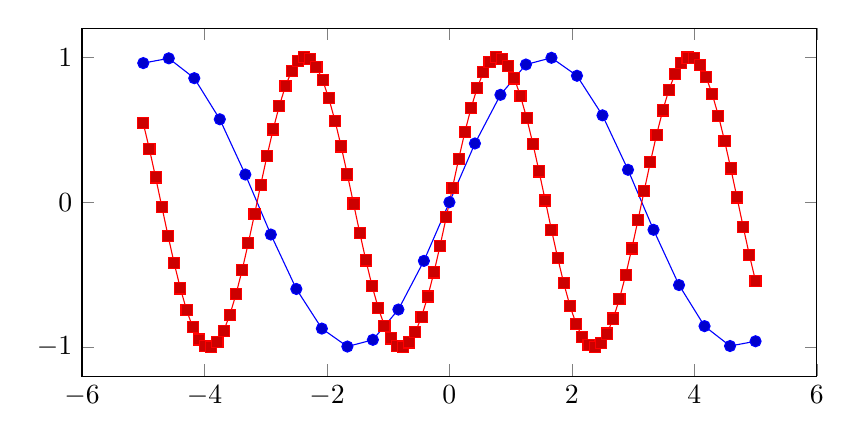
\begin{tikzpicture}
				\begin{axis}[
					width=0.9\textwidth,
					height=6cm,
					]
					
					\addplot {sin(deg(x))};
					\addplot+[samples=100] {sin(deg(2*x))};
				
				\end{axis}
			\end{tikzpicture}
			\caption{A nice sinus plot with Tikz.}
		\end{figure}
	\end{frame}
	
	% FRAME
	\begin{frame}{Bar charts}
		\begin{figure}
			\centering
			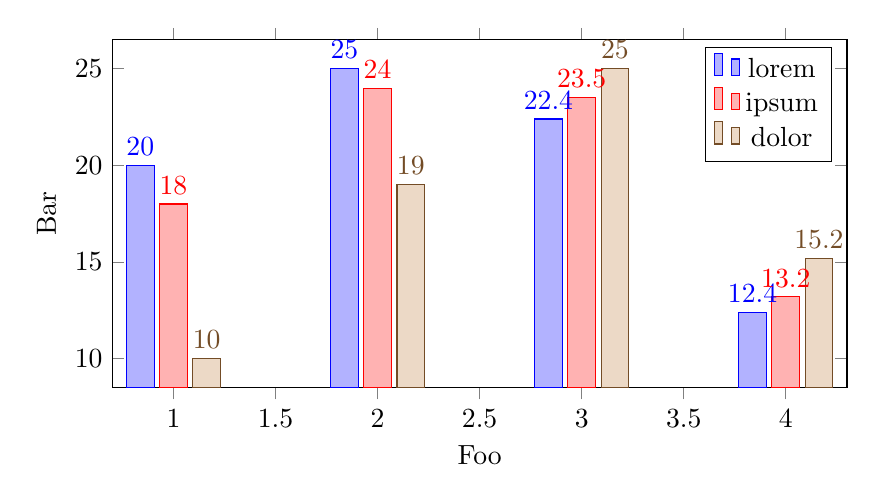
\begin{tikzpicture}
				\begin{axis}[
						ybar,
						xlabel={Foo},
					  	ylabel={Bar},
					  	width=0.9\textwidth,
					  	height=6cm,
						nodes near coords,
						nodes near coords align={vertical},
					]
					
					\addplot plot coordinates {(1, 20) (2, 25) (3, 22.4) (4, 12.4)};
					\addplot plot coordinates {(1, 18) (2, 24) (3, 23.5) (4, 13.2)};
					\addplot plot coordinates {(1, 10) (2, 19) (3, 25) (4, 15.2)};
					
					\legend{lorem, ipsum, dolor}
				
				\end{axis}
			\end{tikzpicture}
			\caption{A nice bar chart with Tikz.}
		\end{figure}
	\end{frame}
	
	% FRAME
	\begin{frame}{Quotes}
		\begin{quote}
			Veni, Vidi, Vici
		\end{quote}
		from Julius Caesar.
	\end{frame}
		
	% FRAME
	\begin{frame}[fragile]{References}
		Some references to showcase \verb|[allowframebreaks]| on next slide~\cite{Knuth92,ConcreteMath,Simpson,Er01,greenwade93}
	\end{frame}

	% % FRAME
	% \begin{frame}{References}
	% 	\bibliography{pres}
	% 	\bibliographystyle{abbrv}
	% \end{frame}

	% FRAME
	\begin{frame}[allowframebreaks]{References}
      \begin{thebibliography}{1}

         \bibitem{Er01}
         P.~Erd{\H o}s.
         \newblock A selection of problems and results in combinatorics.
         \newblock In {\em Recent trends in combinatorics (Matrahaza, 1995)}, pages 1--6. Cambridge Univ. Press, Cambridge, 1995.
         
         \bibitem{ConcreteMath}
         R.~Graham, D.~Knuth, and O.~Patashnik.
         \newblock {\em Concrete mathematics}.
         \newblock Addison-Wesley, Reading, MA, 1989.
         
         \bibitem{greenwade93}
         G.~D. Greenwade.
         \newblock The {C}omprehensive {T}ex {A}rchive {N}etwork ({CTAN}).
         \newblock {\em TUGBoat}, 14(3):342--351, 1993.
         
         \bibitem{Knuth92}
         D.~Knuth.
         \newblock Two notes on notation.
         \newblock {\em Amer. Math. Monthly}, 99:403--422, 1992.
         
         \bibitem{Simpson}
         H.~Simpson.
         \newblock Proof of the {R}iemann {H}ypothesis.
         \newblock preprint (2003), available at \texttt{http://www.math.drofnats.edu/riemann.ps}, 2003.
         
      \end{thebibliography}
   \end{frame}
	
\end{document}
